\documentclass[tikz]{standalone}

\usepackage[T1]{fontenc}
\usepackage[english]{babel}

\usepackage{standalone}

\begin{document}
    \begin{tikzpicture}
    	\node[visible on=<6->] (residual) at (0,0) {\fbox{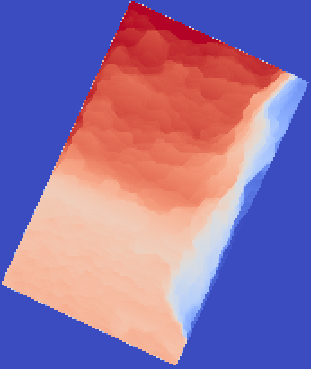
\includegraphics[height=1.5cm, angle=270]{images/introduction/graphical_abstract/residual}}};
        \path (residual.south) node[anchor=north, text width=2.5cm, align=center, visible on=<6->] (residual_legend) {\footnotesize Height based};

        \path (residual.west) + (-1, 0) node[anchor=east, visible on=<3->] (facet_graph) {\includestandalone[mode=buildnew, height=1.5cm]{figures/graphical_abstract/building_graph}};
        \path (residual.west) + (-1, 0) node[anchor=east, visible on=<1-2>, rectangle, fill=white, fit=(facet_graph)] (facet_graph_mask) {};
        \path (facet_graph.south) node[anchor=north, visible on=<3->] (facet_graph_legend) {\footnotesize Geometric};

        \path (residual.east) + (1, 0) node[anchor=west, visible on=<7->] (ortho_projection) {\fbox{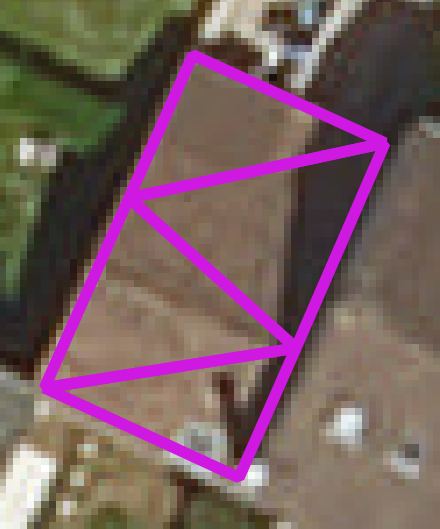
\includegraphics[height=1.5cm, angle=270]{images/introduction/graphical_abstract/orthoprojection}}};
        \path (ortho_projection.south) node[anchor=north, visible on=<7->] (ortho_projection_legend) {\footnotesize Image based};

        \scoped[on background layer]{
            \path (facet_graph.west |- residual.north) + (-1pt, 1pt) node (top_left) {};
            \path (ortho_projection_legend.south east) + (1pt, -1pt) node (down_right) {};
            \node[
                fit=(top_left)(down_right),
                draw,
                rectangle,
                rounded corners,
                visible on=<2->
            ] (frame) {};
            \path (frame.north west) node[anchor=south west, visible on=<2->] (features) {\footnotesize Features};

            \node[
                fit=(facet_graph)(facet_graph_legend |- residual_legend.south),
                fill=green!30,
                rectangle,
                rounded corners,
                visible on=<4->
            ] (intrinsic) {};
            \node[
                fit=(residual)(residual_legend)(ortho_projection)(ortho_projection_legend),
                fill=violet!30,
                rectangle,
                rounded corners,
                visible on=<5->
            ] (extrinsic) {};
        }
        
        \path (frame.north) + (0, 1.5) node[anchor=south, text width=2.5cm, align=center, visible on=<1->] (model_legend) {\footnotesize Input model};
        \path (model_legend.north) node[anchor=south, visible on=<1->] (model) {\includestandalone[mode=buildnew, height=1.5cm]{figures/graphical_abstract/building_model}};

        \path (ortho_projection.east |- model.north) + (1, 0) node (rs_data) {};
        \draw[->, line width=2pt, dashed, visible on=<5->, violet!30] (rs_data) |- (frame.east) node[left, pos=.1, text width=5em, black] {\footnotesize Remote sensing data.};

		\path (frame.south) + (0, -1.5) node[anchor=north, visible on=<8->] (errors) {\includestandalone[mode=buildnew, height=1.5cm]{figures/graphical_abstract/building_errors}};
        \path (errors.south) node[anchor=north, text width=2.5cm, align=center, visible on=<8->] (errors_legend) {\footnotesize Error detection};
        \path (errors.15) + (.4, 0) node[align=center, visible on=<9->] (errors_list) {\footnotesize {\color{red} \(\blacksquare\) \texttt{\acrshort{acr::fib}}}};
        \path (errors_list.south) node[align=center, visible on=<9->] (errors_list) {\footnotesize {\color{green} \(\blacksquare\) \texttt{\acrshort{acr::fos}}}};

        \path[draw, ->, line width=2pt, rounded corners=10pt, IGNGreen, visible on=<2->] (model_legend.south) -- (frame.north);
        \path[draw, ->, line width=2pt, rounded corners=10pt, IGNGreen, visible on=<8->] (frame.south) -- (errors.north) node [midway, left, IGNGreen] {\footnotesize Supervised classifier (RF, SVM)};
    \end{tikzpicture}
\end{document}
